\documentclass{article}
\usepackage[utf8]{inputenc}
\usepackage{tikz}
\usepackage{amsmath}
\usepackage{bm}
\usetikzlibrary{positioning}

\title{8.01 Problem Set 8}
\author{Robert Durfee - Lecture 7 - Table 9}
\date{October 31, 2017}

\begin{document}

\maketitle

\numberwithin{equation}{section}

\section{Exploding Hockey Puck}

There are no external forces, therefore momentum is conserved from before and
after the explosion:
$$m_{i}\vec{v}_{i}=m_{1f}\vec{v}_{1f}+m_{2f}\vec{v}_{2f}$$
Substituting for the known initial and final masses in terms of $m$:
$$m\vec{v}_{i}=\frac{3}{5}m\vec{v}_{1f}+\frac{2}{5}m\vec{v}_{2f}\Rightarrow\vec{v}_{i}=\frac{3}{5}\vec{v}_{1f}+\frac{2}{5}\vec{v}_{2f}$$
Break vector equation up into component form and substituting for
$v_{1f}=\frac{5}{12}v_{i}$:
$$v_{i}\hat{i}=\frac{3}{5}v_{1f}(-\cos(\theta_{1f})\hat{i}+\sin(\theta_{1f})\hat{j})+\frac{2}{5}v_{2f}(\cos(\theta_{2f})\hat{i}-\sin(\theta_{2f})\hat{j})$$
$$v_{i}\hat{i}=-\frac{3}{5}v_{1f}\cos(\theta_{1f})\hat{i}+\frac{2}{5}v_{2f}\cos(\theta_{2f})\hat{i}\Rightarrow
v_{i}=-\frac{1}{4}v_{i}\cos(\theta_{1f})+\frac{2}{5}v_{2f}\cos(\theta_{2f})$$
$$0\hat{j}=\frac{3}{5}v_{1f}\sin(\theta_{1f})\hat{j}-\frac{2}{5}v_{2f}\sin(\theta_{2f})\hat{j}\Rightarrow0=\frac{1}{4}v_{i}\sin(\theta_{1f})-\frac{2}{5}v_{2f}\sin(\theta_{2f})$$
Rearranging to isolate terms:
\begin{equation}
    v_{i}+\frac{1}{4}v_{i}\cos(\theta_{1f})=\frac{2}{5}v_{2f}\cos(\theta_{2f})
\end{equation}
\begin{equation}
    \frac{1}{4}v_{i}\sin(\theta_{1f})=\frac{2}{5}v_{2f}\sin(\theta_{2f})
\end{equation}
Dividing equation 1.2 by equation 1.1:
\begin{equation}
    \frac{\sin(\theta_{1f})}{4+\cos(\theta_{1f})}=\tan(\theta_{2f})
\end{equation}
From the given information, $\theta_{1f}$ can be determined and substituted into
equation 1.3:
$$\tan(\theta_{1f})=\frac{3d/8}{d/2}\Rightarrow\sin(\theta_{1f})=\frac{3}{5},\
\cos(\theta_{1f})=\frac{4}{5}$$
$$\frac{3/5}{4+4/5}=\tan(\theta_{2f})$$
\begin{equation}\frac{1}{8}=\tan(\theta_{2f})\end{equation}
Knowing the horizontal displacement of $m_{2}$:
\begin{equation}
    \tan(\theta_{2f})=\frac{y}{d/2}
\end{equation}
Setting equation 1.4 and 1.5 equal:
$$\frac{1}{8}=\frac{y}{d/2}\Rightarrow\bm{y=\frac{d}{16}}$$

\section{Relative Velocity}

\subsection*{Part A}

A sketch of two possible vectors $\vec{v}_{A}$ and $\vec{V}$ and $\vec{v}_{B}$,
the relative velocity of the point with respect to coordinate system B:
\begin{center}
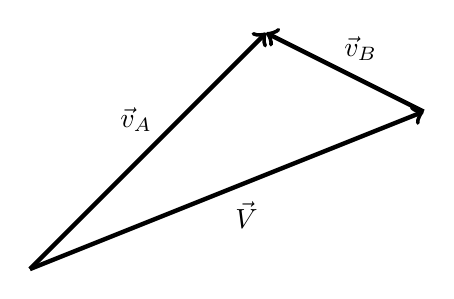
\begin{tikzpicture}
\draw[ultra thick, ->] (-1,-1) -- (2,2) node[pos=0.45, above=0.25]
    {$\vec{v}_{A}$};
\draw[ultra thick, <-] (2,2) -- (4,1) node[pos=0.6, above=0.1] {$\vec{v}_{B}$};
\draw[ultra thick, ->] (-1,-1) -- (4,1) node[pos=0.55, below=0.1] {$\vec{V}$};
\end{tikzpicture}
\end{center}
Therefore, using vector mathematics, $\vec{v}_B$ can be solved for:
\begin{equation}
\vec{v}_{A}=\vec{V}+\vec{v}_{B}\Rightarrow\bm{\vec{v}_{B}=\vec{v}_{A}-\vec{V}}
\end{equation}

\subsection*{Part B}

At the extreme positions during the path of points A and B, it is easy to see
what the relative velocities are graphically. For example, at $\theta=0$ (where
$\vec{v}_{A}=\omega l \hat{i}$ and $\vec{v}_{B}=-\omega l \hat{i}$):
\begin{center}
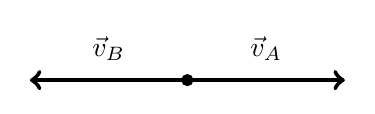
\begin{tikzpicture}
\draw[ultra thick, ->] (0,0) -- (-2,0) node[midway, above=0.1] {$\vec{v}_{B}$};
\draw[ultra thick, ->] (0,0) -- (2,0) node[midway, above=0.1] {$\vec{v}_{A}$};
\filldraw[black] (0,0) circle (2pt);
\end{tikzpicture}
\end{center}
The relative velocities are:
$$\vec{v}_{AB}=2 \omega l\hat{i}, \ \vec{v}_{BA}=-2 \omega l\hat{i}$$ 
Modifying equation 2.1 to fit this problem shows this solution mathematically:
\begin{equation}\vec{v}_{A}-\vec{v}_{B}=\vec{v}_{AB}\end{equation}
\begin{equation}-\vec{v}_{A}+\vec{v}_{B}=\vec{v}_{BA}\end{equation}
Defining $\vec{v}_{A}$ and $\vec{v}_{B}$ in terms of $\omega$, $l$, and $\theta$:
\begin{equation}\vec{v}_{A}=\omega
l\left[\cos(\theta)\hat{i}-\sin(\theta)\hat{j}\right]\end{equation}
\begin{equation}\vec{v}_{B}=\omega
l\left[-\cos(\theta)\hat{i}-\sin(\theta)\hat{j}\right]\end{equation}
Substituting equations 2.4 and 2.5 into equation 2.2:
$$\left[\omega
l\left(\cos(\theta)\hat{i}-\sin(\theta)\hat{j}\right)\right]-\left[\omega
l\left(-\cos(\theta)\hat{i}-\sin(\theta)\hat{j}\right)\right]=\vec{v}_{AB}\Rightarrow\bm{\vec{v}_{AB}=2\omega
l \cos(\theta)\hat{i}}$$

\section{Ping-Pong Ball and Bowling Ball Collision}

Velocities prior to collision:
\begin{center}
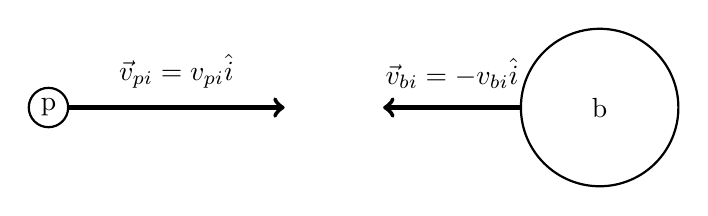
\begin{tikzpicture}
\draw[black, thick] (3.5,0) circle (1) node[] {b};
\draw[black, thick] (-3.5,0) circle (0.25) node[] {p};
\draw[ultra thick, ->] (2.5,0) -- (0.75,0) node[midway, above=0.1]
    {$\vec{v}_{bi}=-v_{bi}\hat{i}$};
\draw[ultra thick, ->] (-3.25,0) -- (-0.5,0) node[midway, above=0.1]
    {$\vec{v}_{pi}=v_{pi}\hat{i}$};
\end{tikzpicture}
\end{center}
Initial relative velocity of the ping-pong ball with respect to the bowling
ball:
$$\vec{v}_{pi}-\vec{v}_{bi}=\vec{v}_{pbi}\Rightarrow
v_{pi}\hat{i}+v_{bi}\hat{i}=\vec{v}_{pbi}$$
Velocities after collision given $m_{b}\gg m_{p}$:
\begin{center}
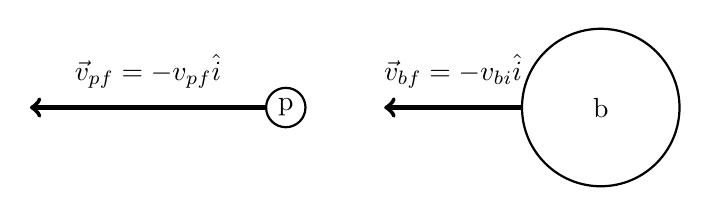
\begin{tikzpicture}
\draw[black, thick] (3.5,0) circle (1) node[] {b};
\draw[black, thick] (-0.50,0) circle (0.25) node[] {p};
\draw[ultra thick, ->] (2.5,0) -- (0.75,0) node[midway, above=0.1]
    {$\vec{v}_{bf}=-v_{bi}\hat{i}$};
\draw[ultra thick, <-] (-3.75,0) -- (-0.75,0) node[midway, above=0.1]
    {$\vec{v}_{pf}=-v_{pf}\hat{i}$};
\end{tikzpicture}
\end{center}
Final relative velocity of the ping-pong ball with respect to the bowling ball:
$$\vec{v}_{pf}-\vec{v}_{bf}=\vec{v}_{pbf}\Rightarrow\vec{v}_{pf}+v_{bi}\hat{i}=\vec{v}_{pbf}$$
Knowing that the relative velocities reverse direction after the collision:
$$\vec{v}_{pbi}=-\vec{v}_{pbf}\Rightarrow v_{pi}\hat{i}+v_{bi}\hat{i}=-(\vec{v}_{pf}+v_{bi}\hat{i})$$
$$\bm{\vec{v}_{pf}=-({v}_{pi}+2v_{bi})\hat{i}}$$

\section{Satellite Fly-By}

Velocities prior to 'collision':
\begin{center}
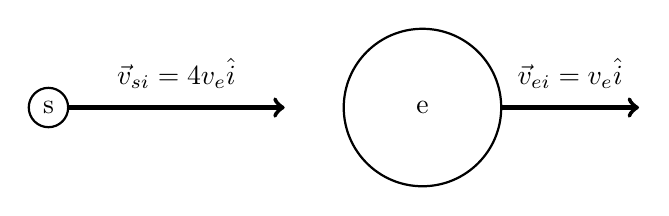
\begin{tikzpicture}
\draw[black, thick] (1.25,0) circle (1) node[] {e};
\draw[black, thick] (-3.5,0) circle (0.25) node[] {s};
\draw[ultra thick, <-] (4,0) -- (2.25,0) node[midway, above=0.1]
    {$\vec{v}_{ei}=v_{e}\hat{i}$};
\draw[ultra thick, ->] (-3.25,0) -- (-0.5,0) node[midway, above=0.1]
    {$\vec{v}_{si}=4v_{e}\hat{i}$};
\end{tikzpicture}
\end{center}
Initial relative velocity of the satellite with respect to the Earth:
$$\vec{v}_{si}-\vec{v}_{ei}=\vec{v}_{sei}\Rightarrow4v_{e}\hat{i}-v_{e}\hat{i}=\vec{v}_{sei}$$
Velocities after 'collision' given $m_{e}\gg m_{s}$:
\begin{center}
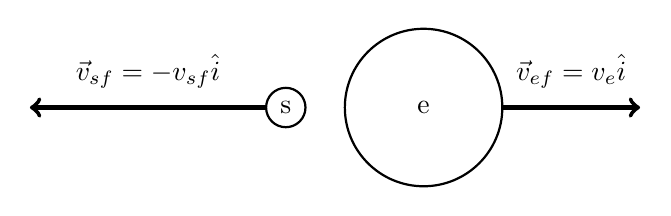
\begin{tikzpicture}
\draw[black, thick] (1.25,0) circle (1) node[] {e};
\draw[black, thick] (-0.50,0) circle (0.25) node[] {s};
\draw[ultra thick, <-] (4,0) -- (2.25,0) node[midway, above=0.1]
    {$\vec{v}_{ef}=v_{e}\hat{i}$};
\draw[ultra thick, <-] (-3.75,0) -- (-0.75,0) node[midway, above=0.1]
    {$\vec{v}_{sf}=-v_{sf}\hat{i}$};
\end{tikzpicture}
\end{center}
Final relative velocity of the satellite with respect to the Earth:
$$\vec{v}_{sf}-\vec{v}_{ef}=\vec{v}_{sef}\Rightarrow\vec{v}_{sf}-v_{e}\hat{i}=\vec{v}_{sef}$$
Knowing that the relative velocities reverse direction after the 'collision':
$$\vec{v}_{sei}=-\vec{v}_{sef}\Rightarrow4v_{e}\hat{i}-v_{e}\hat{i}=-(\vec{v}_{sf}-v_{e}\hat{i})$$
$$\bm{\vec{v}_{sf}=-2v_{e}\hat{i}}$$


\end{document}
